% CVPR 2022 Paper Template
% based on the CVPR template provided by Ming-Ming Cheng
% modified and extended by Stefan Roth

\documentclass[10pt,twocolumn,letterpaper]{article}

\usepackage[pagenumbers]{cvpr}

\usepackage{graphicx}
\usepackage{amsmath}
\usepackage{amssymb}
\usepackage{booktabs}
\usepackage[pagebackref,breaklinks,colorlinks]{hyperref}
\usepackage[capitalize]{cleveref}

\crefname{section}{Sec.}{Secs.}
\Crefname{section}{Section}{Sections}
\Crefname{table}{Table}{Tables}
\crefname{table}{Tab.}{Tabs.}

\def\cvprPaperID{0}
\def\confName{CSE 559a}
\def\confYear{\the\year{}}

\begin{document}

\title{LensLab: A TCP-Based Unity/OpenCV Pipeline for Live ChArUco AR}

\author{
Julie Yang
}
\maketitle

\begin{abstract}
LensLab is a live augmented reality prototype that connects an OpenCV-based
camera and pose estimation pipeline with a Unity runtime.  The system uses a
printed ChArUco target as a calibrated reference object.  Python captures live
camera frames, detects ChArUco corners, calibrates camera intrinsics, estimates
the target pose with PnP, and streams both camera images and pose metadata to
Unity over TCP.  Unity loads the shared calibration JSON, applies a calibrated
projection matrix, renders the live camera frame as a world-space background
plane, and anchors virtual content on the detected board.  The final design was
the result of an iterative development process: I first validated the geometry
offline on CPU, then built a JSON calibration contract, then implemented a
separate Unity AR validation path, and finally replaced direct Unity-side camera
capture with a Python-owned TCP publisher after performance bottlenecks became
the main obstacle.  The resulting prototype demonstrates a practical real-time
AR loop while keeping the calibration, pose estimation, and rendering stages
inspectable.
\end{abstract}

\section{Introduction}

The goal of this project is to build a small but complete augmented reality
pipeline without relying on a mobile AR framework.  Instead of treating
calibration and tracking as hidden services, LensLab exposes each step: camera
calibration, distortion modeling, pose estimation, camera projection matching,
and final Unity rendering.  This makes the project useful both as a working AR
demo and as an engineering study of how computer vision outputs can be brought
into a game engine.

The target object is a ChArUco board, which combines ArUco marker identities
with chessboard-like corner localization.  This target is convenient for a
course project because it supports robust detection under partial visibility and
also provides metric structure for camera calibration and pose estimation.  The
main output of the Python side is a shared calibration file containing image
size, focal lengths, principal point, OpenCV rational distortion coefficients,
and board metadata.  During runtime, the Python process estimates the board pose
for each camera frame and sends the current frame and pose to Unity.

The final system has two main workflows.  First, the user runs live calibration
from Python, manually accepts stable ChArUco observations, and writes
\texttt{camera\_calibration.json}.  Second, the user opens Unity, creates a live
AR scene from a menu command, and presses Play.  Unity starts the Python pose
server, receives a TCP stream, displays the live camera feed, and drives virtual
content from the latest pose.

The most important design choice is that Python owns the webcam in the final
runtime.  An earlier Unity-owned camera design was simpler conceptually, but it
was not fast enough on Windows for the desired interactive result.  OpenCV can
request MJPG capture directly from the camera, while Unity's \texttt{WebCam}
path was difficult to make reliable at high resolution and frame rate.  Moving
camera ownership to Python and using TCP as the Unity boundary made the system
less monolithic, but substantially more stable.

\section{Related Work}

LensLab builds on classical camera calibration and pose estimation.  Zhang's
calibration method established the practical use of planar calibration targets
for estimating camera intrinsics from multiple views~\cite{Zhang2000}.  OpenCV
implements these ideas and provides camera calibration, distortion models,
projection utilities, and PnP solvers~\cite{OpenCV}.  For target detection, the
project uses ArUco-style fiducials and ChArUco boards, which combine marker
identification with chessboard corner interpolation~\cite{GarridoJurado2014}.

The rendering side follows the standard AR requirement that the virtual camera
must match the physical camera.  In practice, this means converting the
calibrated focal lengths and principal point into a Unity projection matrix and
placing rendered content in the coordinate frame implied by the OpenCV pose.
Unity provides the real-time rendering environment and scene graph used for the
final display~\cite{Unity}.  The contribution of this project is not a new
calibration or pose algorithm, but rather a complete bridge from these computer
vision components into an interactive Unity scene.

\section{Approach}

\subsection{Development trajectory}

The project progressed through several stages.  The first stage was a CPU-only
OpenCV validation path.  In this stage, the main question was whether the board
could be detected reliably and whether the calibration output was numerically
reasonable.  The second stage introduced a calibration JSON contract.  This was
important because Unity and Python need to agree on image size, intrinsics,
distortion parameters, and board dimensions.  A stable file format made it
possible to debug the two sides independently.

The third stage implemented a separate Unity AR validation path.  Unity loaded
the calibration JSON, applied a calibrated camera projection, and rendered
content using pose data exported from Python.  This confirmed that the
coordinate conversion and projection mapping were approximately correct before
any live networking was introduced.

The fourth stage attempted to integrate Python more directly into the Unity
runtime.  This exposed a practical problem: Unity's frame update model and
camera capture behavior made it difficult to keep live image acquisition,
OpenCV processing, and Unity rendering synchronized at an acceptable frame
rate.  The final stage therefore changed the architecture.  Python became a
publisher process that owns the camera and broadcasts the newest frame and pose
to Unity over TCP.  Unity became a subscriber and renderer.  This separation
reduced latency accumulation and made each component easier to reason about.

\subsection{Live ChArUco calibration}

The live calibration tool opens the camera with OpenCV, detects markers, and
interpolates ChArUco corners.  The user accepts frames manually when the board
is visible and stable.  After enough accepted observations are collected, OpenCV
estimates camera intrinsics and distortion coefficients.  The output JSON is
then copied into Unity Resources so that the runtime and the Python server use
the same calibration.

\begin{figure}[t]
    \centering
    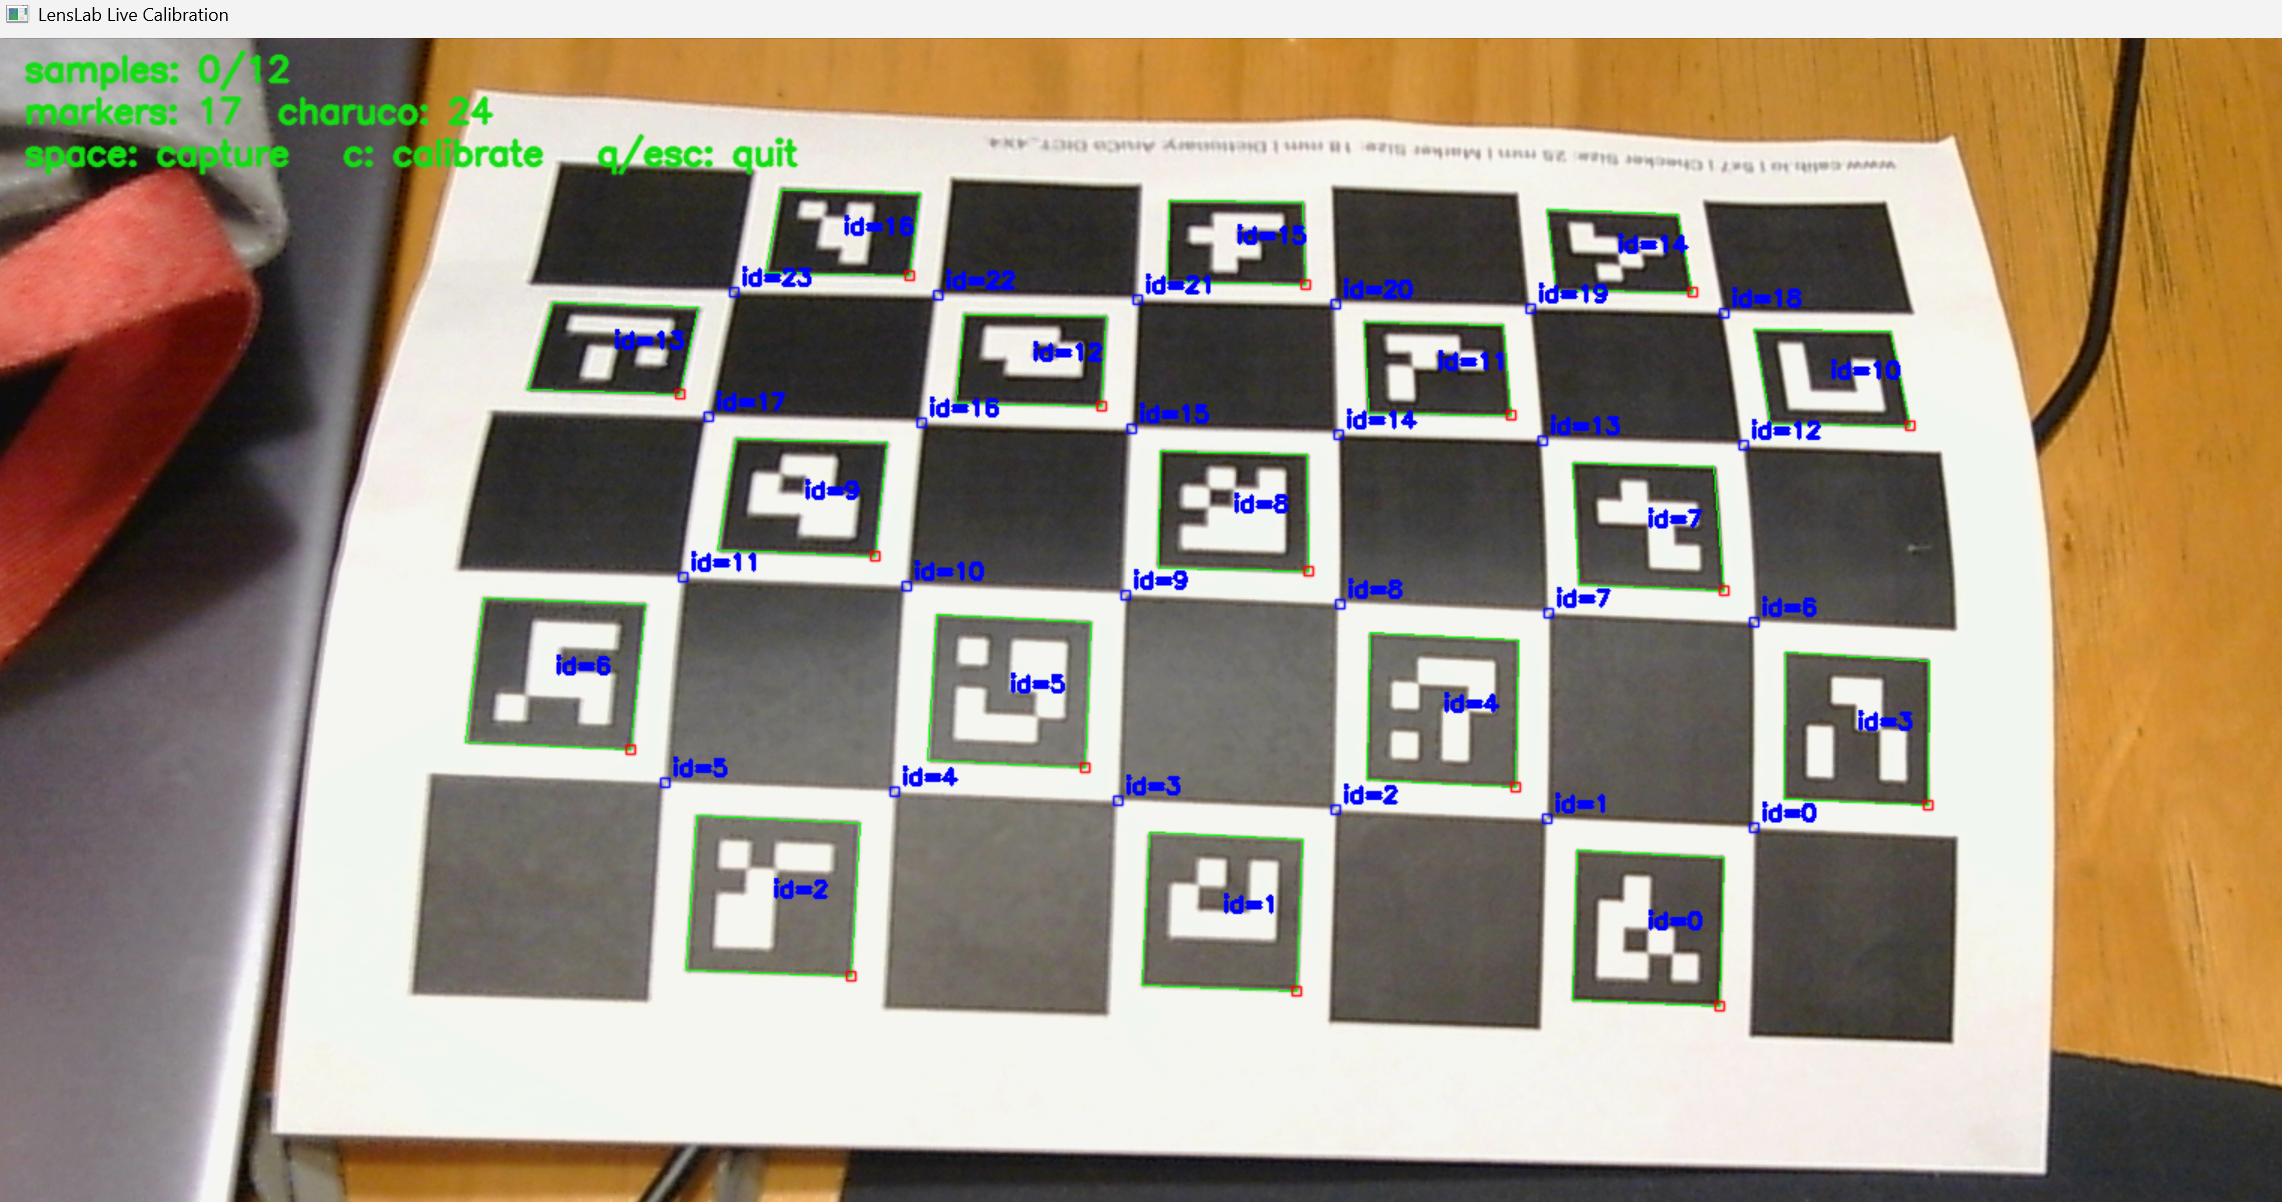
\includegraphics[width=\linewidth]{pic-1-CreateCalibrationJson.png}
    \caption{Live ChArUco calibration interface.  The overlay shows detected
    ArUco markers, interpolated ChArUco corners, and the number of accepted
    calibration samples.}
    \label{fig:calibration}
\end{figure}

The calibration file contains the image resolution, focal lengths
$(f_x, f_y)$, principal point $(c_x, c_y)$, distortion coefficients, and target
metadata.  The ideal pinhole projection before distortion is
\begin{equation}
    \begin{bmatrix} u \\ v \\ 1 \end{bmatrix}
    \sim
    \begin{bmatrix}
    f_x & 0 & c_x \\
    0 & f_y & c_y \\
    0 & 0 & 1
    \end{bmatrix}
    \begin{bmatrix} X/Z \\ Y/Z \\ 1 \end{bmatrix}.
\end{equation}
Unity uses these intrinsics to build a matching camera projection rather than
using an arbitrary field of view.

\subsection{TCP pose server}

The final runtime server is implemented in \texttt{pose\_server.py}.  It opens
the webcam through OpenCV, requests MJPG capture, detects the ChArUco board, and
solves for pose.  A key engineering detail is that the server broadcasts only
the latest frame to each client.  Each client has a single-slot mailbox.  If
Unity is slower than the camera, old frames are overwritten instead of queued.
This avoids the common failure mode where a real-time system remains high-FPS
internally but displays increasingly stale frames.

The TCP message format is deliberately simple:
\begin{equation}
\texttt{uint32 jpeg\_len} \; || \; \texttt{jpeg bytes} \; || \;
\texttt{uint32 json\_len} \; || \; \texttt{pose json}.
\end{equation}
The pose JSON includes whether the board was detected, the number of markers
and ChArUco corners, the OpenCV rotation and translation vectors, a flattened
rotation matrix, and the reprojection error.  The server requires at least six
ChArUco correspondences before calling iterative PnP, because OpenCV's DLT
initialization requires at least six 3D-2D point pairs.  Frames with fewer
corners are treated as non-detections rather than runtime errors.

\subsection{Unity runtime}

\begin{figure}[t]
    \centering
    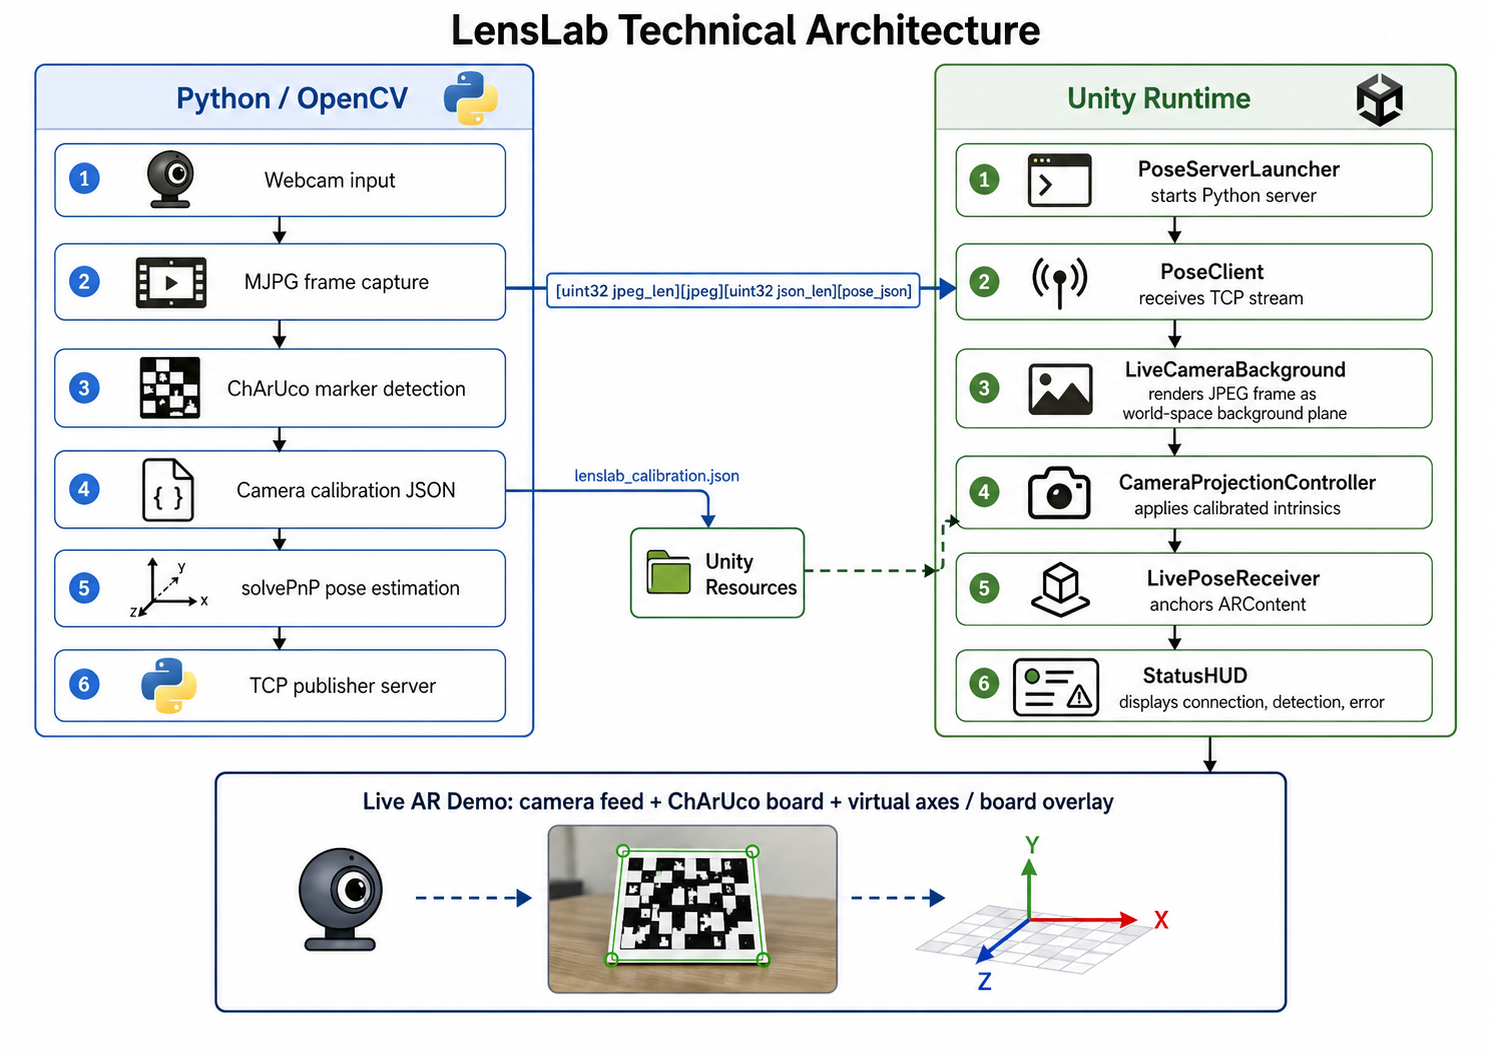
\includegraphics[width=\linewidth]{architecture.png}
    \caption{Final LensLab architecture.  Python owns the camera and pose
    estimation; Unity owns rendering and scene interaction.  The boundary
    between the two systems is a TCP stream containing the latest JPEG frame and
    pose JSON.}
    \label{fig:architecture}
\end{figure}

The Unity runtime is organized as a small plugin.  The editor menu creates the
demo hierarchy automatically.  \texttt{LensLabPoseServerLauncher} starts and
stops the Python server when Play mode begins and ends.
\texttt{LensLabPoseClient} connects to the server on localhost, reads the
length-prefixed stream on a background thread, and decodes the newest JPEG on
the main Unity thread.  This thread split is important because Unity APIs such
as texture updates and JSON deserialization must remain on the main thread.

\texttt{LensLabLiveCameraBackground} binds the latest received texture to a
world-space background plane in front of the Unity camera.  This is preferable
to drawing the camera image in a screen-space overlay, because an overlay would
cover all 3D AR content.  With a world-space background, virtual content between
the camera and the background plane naturally appears in front of the live
image.  \texttt{LensLabLivePoseReceiver} converts the OpenCV pose into Unity
camera space and drives the AR content transform.  A small HUD reports TCP
connection status, board detection status, number of detected corners, and
current reprojection error.

\begin{figure}[t]
    \centering
    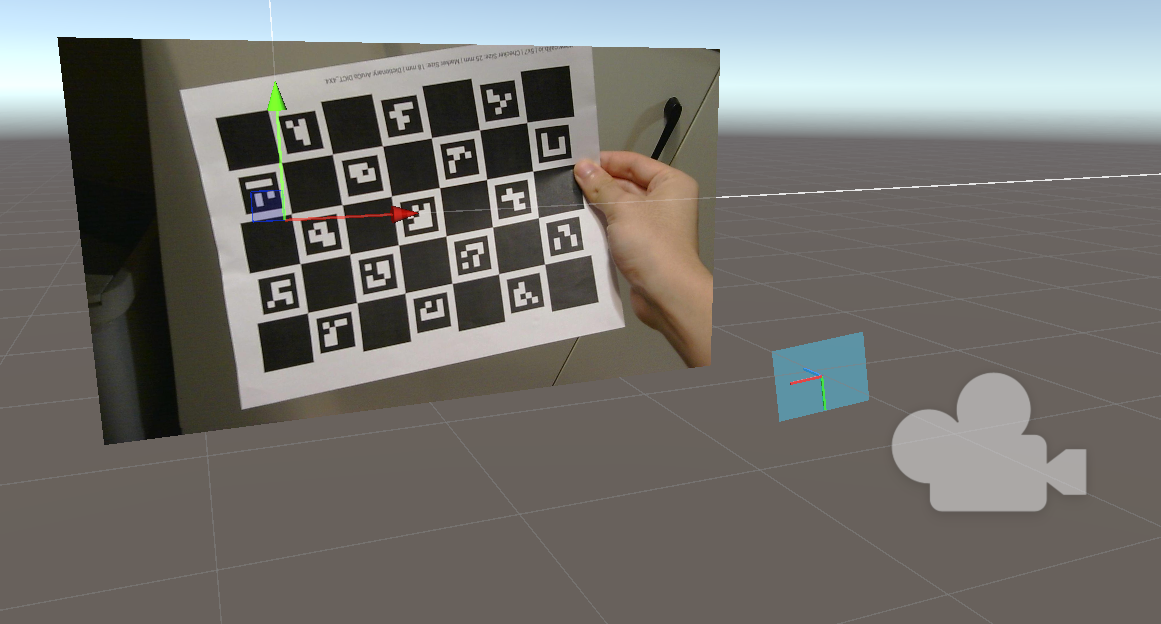
\includegraphics[width=\linewidth]{pic-3-ARObjectIn3DScene.png}
    \caption{Unity scene view showing the live camera image as a world-space
    background plane and AR content positioned in front of it.}
    \label{fig:sceneview}
\end{figure}

\section{Results}

The final demo was tested on Windows using Unity 2022.3, Python 3.10, and
\texttt{opencv-contrib-python}.  The ChArUco board used a 7 by 5 square layout
with 25 mm squares and 18 mm markers.  The live calibration interface detected
markers and corners interactively as shown in \cref{fig:calibration}.  The
runtime server then used the same board definition and calibration file for
pose estimation.

\begin{figure}[t]
    \centering
    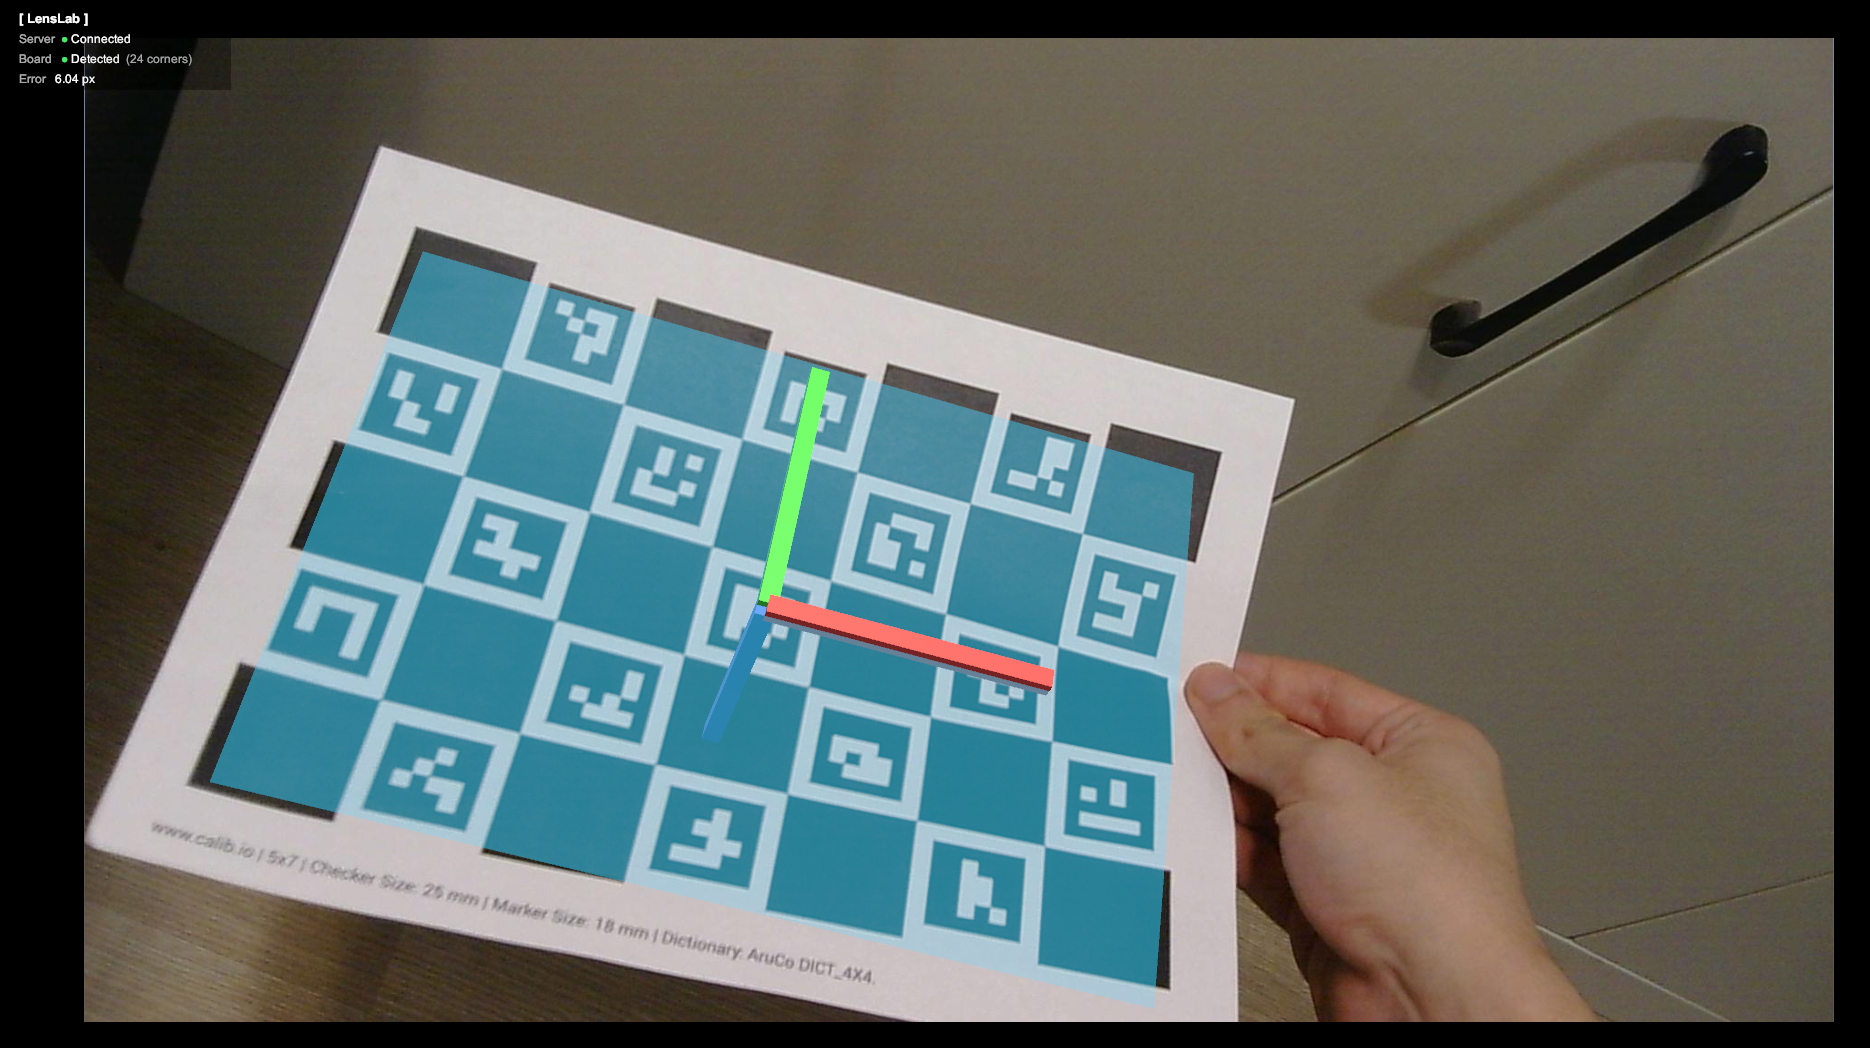
\includegraphics[width=\linewidth]{pic-2-GameView.png}
    \caption{Final Unity Game view.  The HUD reports that the TCP server is
    connected and the board is detected.  The translucent board overlay and
    colored pose axes are rendered over the live camera frame.}
    \label{fig:gameview}
\end{figure}

\Cref{fig:gameview} shows the final AR output.  The camera image is streamed
from Python to Unity, while the board overlay and coordinate axes are rendered
as Unity objects.  In the captured example, the HUD reports 24 detected
ChArUco corners and a reprojection error of approximately 6 pixels.  This value
is not a full benchmark, but it is a useful runtime diagnostic: when the target
is clearly visible, the system reports a stable detection and keeps the virtual
content attached to the board.

The most significant qualitative result is that the final system remains
interactive after the architecture switch.  In the earlier Unity-owned camera
path, the camera feed could freeze or update too slowly, which prevented
convincing AR output.  In the TCP publisher design, Python can negotiate camera
capture through OpenCV and Unity only consumes the latest available frame.  This
keeps the rendered display responsive and avoids unbounded latency.

The current implementation is still a prototype.  It does not include formal
pose accuracy measurement against an external tracking system, and the virtual
content is intentionally simple: a board-aligned translucent quad and coordinate
axes.  However, this simplicity is useful for validation because visual errors
are easy to see.  Misalignment usually indicates either calibration mismatch,
insufficient board visibility, or a coordinate conversion issue.

\section{Discussion and Conclusions}

The main lesson from this project is that a working AR pipeline depends as much
on systems integration as on the underlying vision algorithms.  Camera
calibration and PnP are well-supported in OpenCV, but bringing their outputs
into Unity required careful handling of data formats, coordinate systems,
threading, camera ownership, and rendering order.

The development process also showed why early validation stages were useful.
The CPU-only OpenCV stage made it possible to confirm marker detection and
calibration independently.  The calibration JSON stage created a stable
contract between Python and Unity.  The separate Unity validation stage exposed
projection and coordinate issues before live performance became a confounding
factor.  Finally, the failed direct integration attempt was still valuable
because it revealed the real bottleneck: camera acquisition and frame update
behavior, not the mathematics of pose estimation.

The final TCP architecture is not the most polished packaging solution, but it
is a practical engineering compromise.  It gives Python full control of camera
capture and OpenCV processing while letting Unity focus on rendering and user
interaction.  Future work could package the Python server as an executable,
add stronger pose smoothing, record evaluation videos, and replace the simple
debug axes with richer AR content.  A more rigorous evaluation could also
measure pose jitter and alignment error across board distances and viewing
angles.

\section{Statement of Individual Contribution}

This was an individual project.  I implemented the live ChArUco calibration
pipeline, the calibration JSON contract, the Python pose server, the TCP stream
format, the Unity runtime components, the automatic scene creation menu, the
HUD, debugging utilities, and the final report.  I also collected the test
images and screenshots used to demonstrate the system.

\section{External Resources Used}

The project uses OpenCV and \texttt{opencv-contrib-python} for camera capture,
ArUco/ChArUco detection, calibration, distortion modeling, and PnP pose
estimation~\cite{OpenCV}.  NumPy is used for numerical array handling, and
PyYAML is used for reading the board configuration file.  Unity 2022.3 is used
for rendering, scene management, editor tooling, and the final AR display
runtime~\cite{Unity}.  The report uses the CVPR 2022 LaTeX template.  The
ChArUco target is based on OpenCV's ArUco/ChArUco board implementation and the
published ArUco marker work~\cite{GarridoJurado2014}.

The main external resources are:
\begin{itemize}
    \item OpenCV documentation: \url{https://docs.opencv.org/}
    \item OpenCV Python package: \url{https://pypi.org/project/opencv-contrib-python/}
    \item Unity Manual: \url{https://docs.unity3d.com/Manual/}
    \item NumPy: \url{https://numpy.org/}
    \item PyYAML: \url{https://pyyaml.org/}
    \item CVPR LaTeX template: \url{https://github.com/cvpr-org/author-kit}
\end{itemize}

{\small
\bibliographystyle{ieee_fullname}
\bibliography{bibliography}
}

\end{document}
